\section{Ph.D. Route}
\label{res-des-sec:phd-route}

A good way to present the methodological route of this research project is by knowing my Ph.D. route. I divide my Ph.D. study into three phases, describing the project structuring (Section \ref{phd-route-ss:proj-str}), the pre- and in-intervention (Section \ref{phd-route-ss:pre-int} and \ref{phd-route-ss:in-int}), and the analysis and discussion (Section \ref{phd-route-ss:ana-dis}). I scheme this route in Figure \ref{fig:phd-route}.

\begin{figure}[ht!]
\centering

\caption{\textmd{Schema of \acrshort{PBL} By-Cycles Framework using the Deming cycle (\acrshort{PDCA}) structure.}}
\label{fig:pbl-by-cycles}
\fcolorbox{gray}{white}{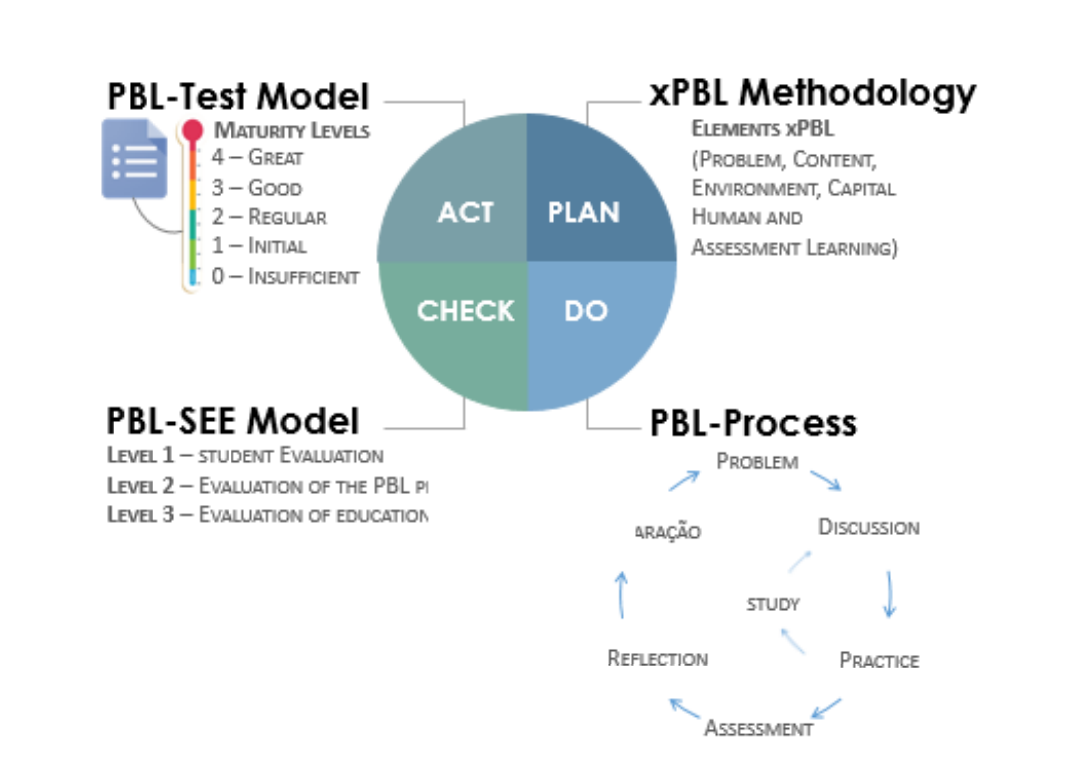
\includegraphics[width=0.9\textwidth]{images/chapter-07/pbl-by-cycles.png}}

\par\medskip\ABNTEXfontereduzida\selectfont\textbf{Source:} \citeonline[p.~60]{alexandre:2018}.
\end{figure}

\begin{figure}[ht!]
\centering

\caption{\textmd{Schema presenting my \acrshort{Ph.D.} route composed of three big phases: (i) project structuring, (ii) pre- and in-intervention, and (iii) analysis \& discussion.}}
\label{fig:phd-route}
\fcolorbox{gray}{white}{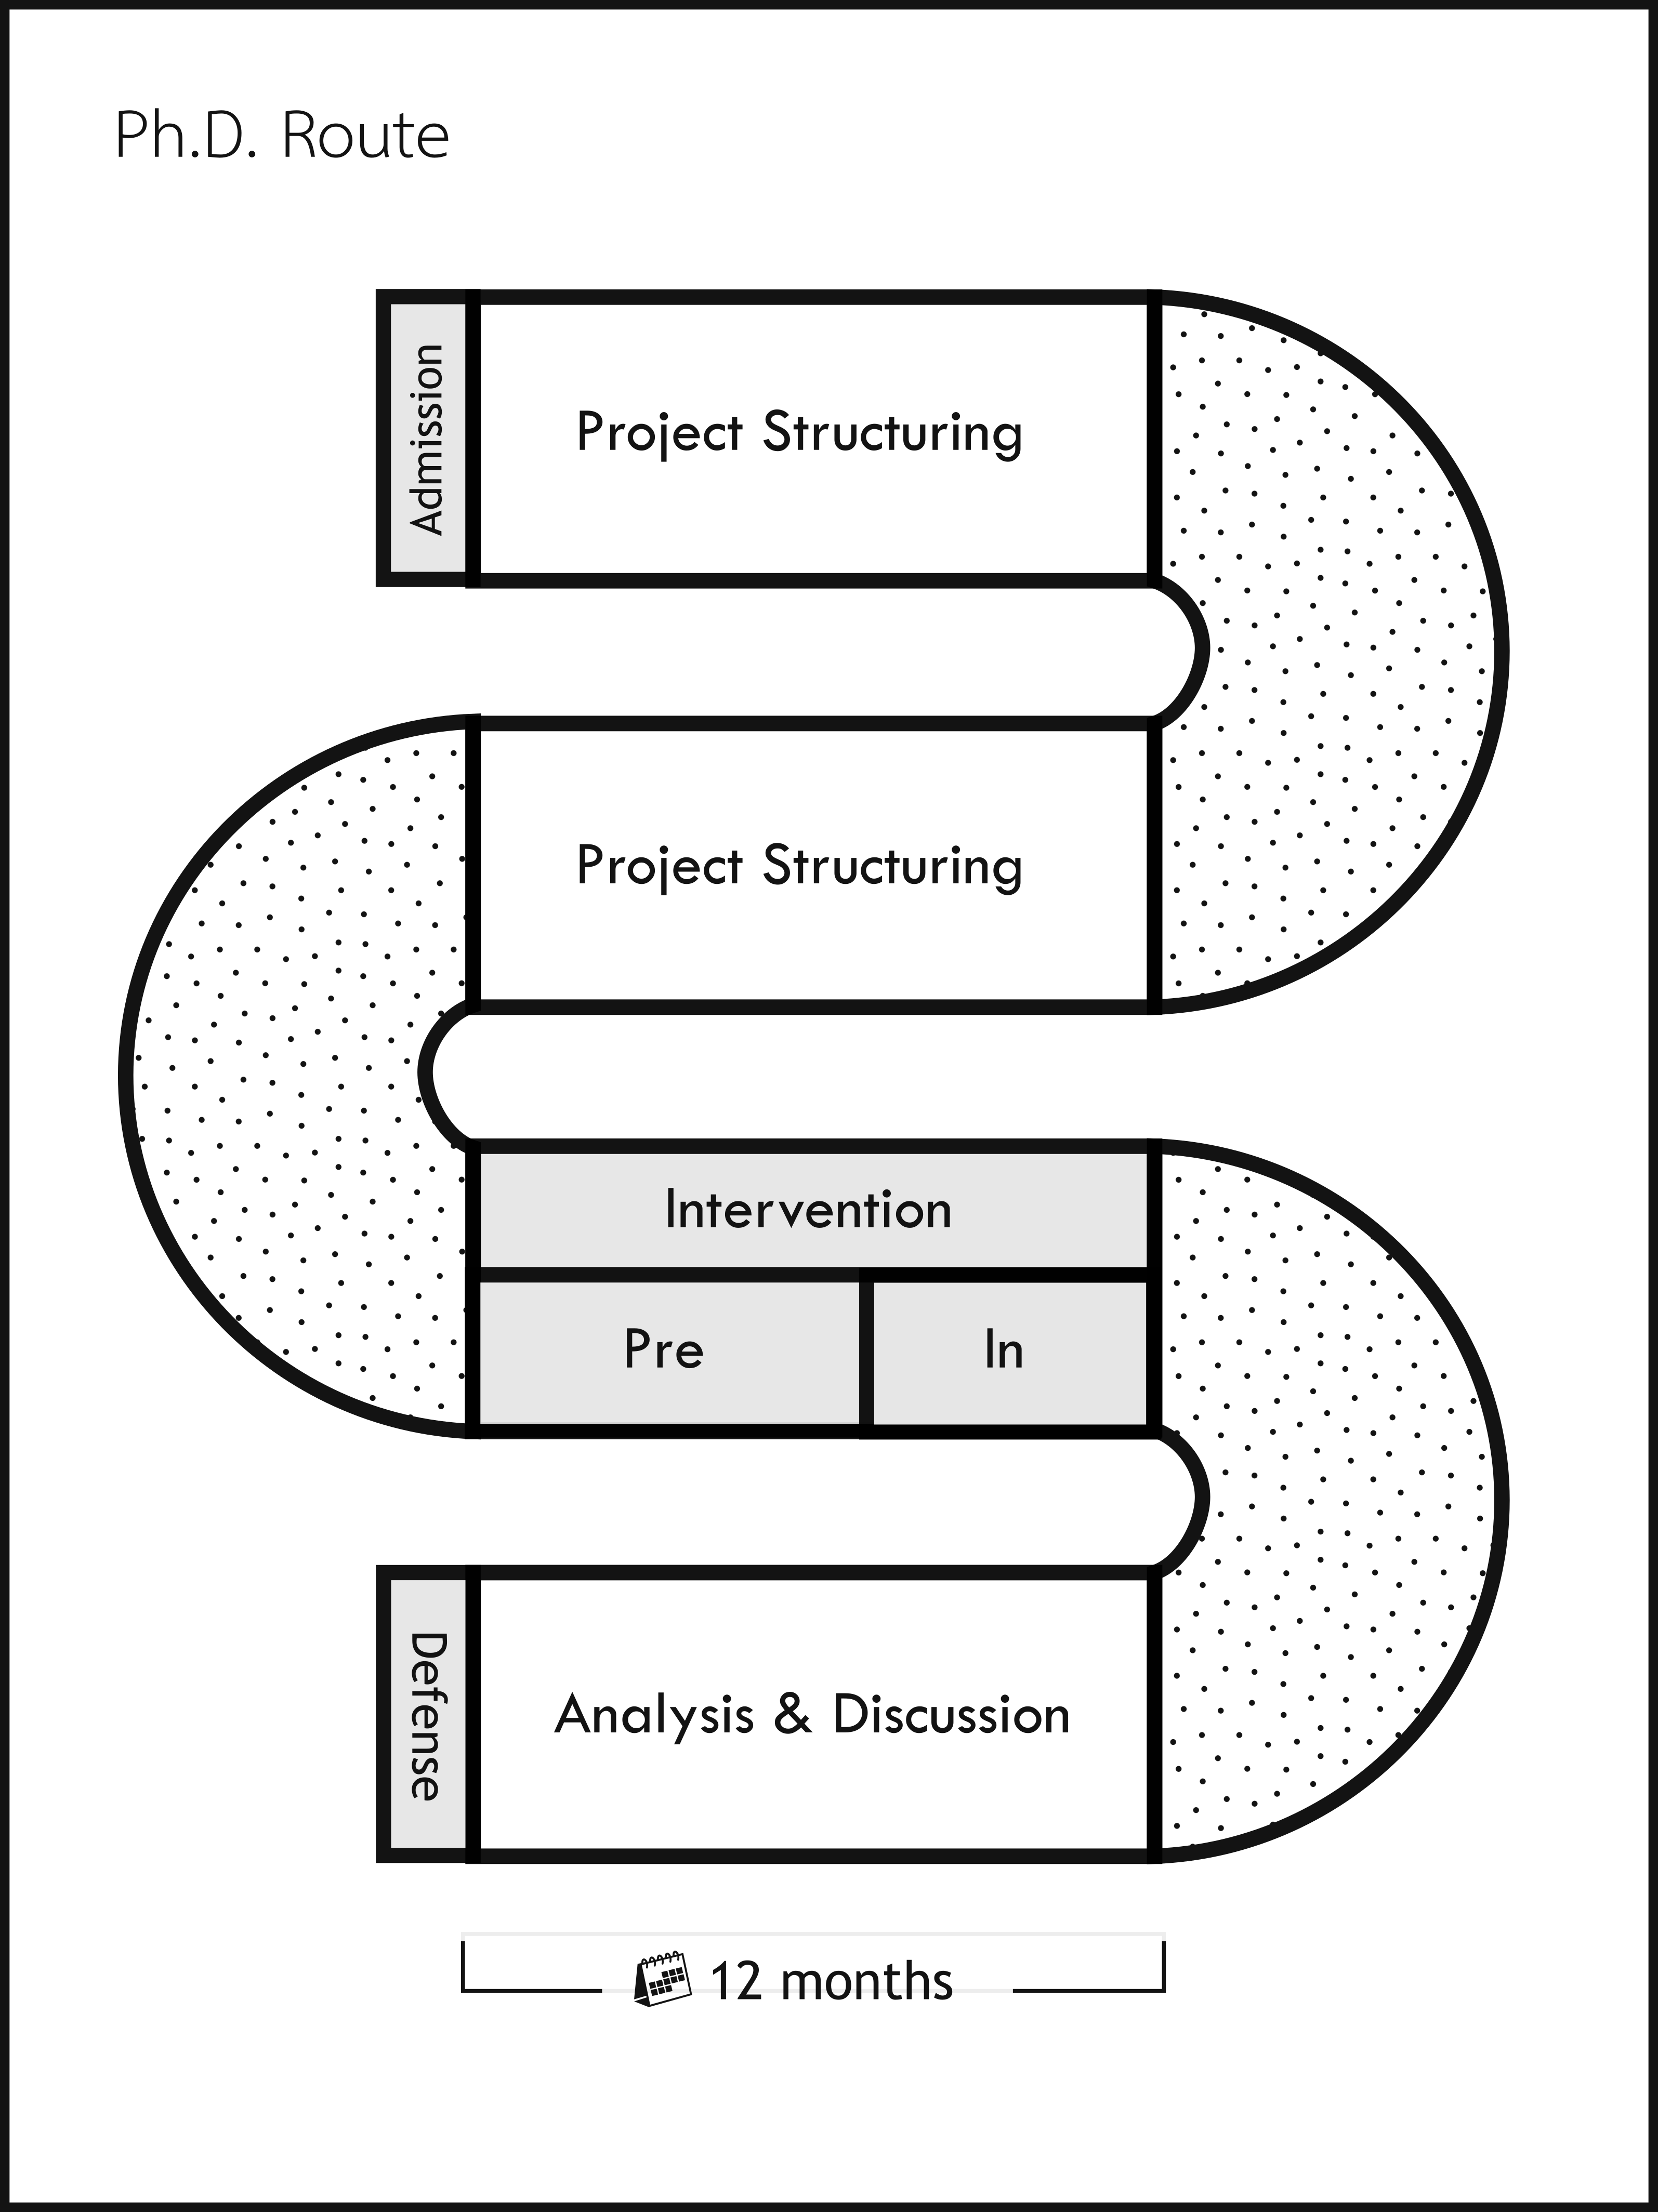
\includegraphics[width=0.9\textwidth]{images/chapter-07/phd-route.png}}

\par\medskip\ABNTEXfontereduzida\selectfont\textbf{Source:} Created by the author (2024).
\end{figure}

\subsection{Project Structuring}
\label{phd-route-ss:proj-str}

The first phase covers all activities and decisions responsible for helping structure the research project. This phase lasted nearly 24 months, comprehending from my admission to the \gls{Ph.D.} program (October 2020) until the qualifying exam (November 2022). I list the main activities that are: attended courses, reading tasks, tutoring, paper writing, and qualifying project. I will describe each of them in detail as follows.

My advisor and I decided on a set of introductory courses that would help me in this phase. The major part was related to research methodology: (i) “Research in Computing Science”, (ii) “Evidence-based Software Engineering”, and (iii) “Qualitative Research in Software Engineering”. I attended all of them at \gls{CIn}. Beyond these, a strategic course was “Education and Society” that I had the opportunity to attend at the \gls{UFPE} Education Center. These four courses gave me incredible constructs to structure Chapters \ref{chap:rel-work}, \ref{chap:reflex-essay}, and \ref{chap:res-methodology} of this research.

Another crucial activity during this phase was my readings. Although part of my academic journey as a professor provided me with previous knowledge about active learning in \acrfull{CSE} area, I needed to deepen my research about \gls{SDL} and equity concepts. This activity pervaded the whole project structuring (and part of other \gls{Ph.D.} route phases), having the Chapters \ref{chap:intro}, \ref{chap:sdl}, and \ref{chap:equity} as the more visible results.

Bearing to know the potential field of data collection, I helped my advisor (and my colleague-tutors) during the integrated \gls{PBL} approach (Section \ref{res-des-sec:context}) as a tutor during the 2020.2 academic term (from May to September 2021). This opportunity allowed me to understand the \gls{PBL} By-Cycles Framework \cite{alexandre:2018} in more detail, observing all the possibilities to intersect my research interests into a context in which the \gls{PBL} in \gls{CSE} achieved a high level of maturity \cite{santos:2013}. The first outline of the research design arose during these tutoring moments.

Not all doctoral credits are offered as courses in a classical format. A part of them can be conducted through individual mentoring between an advisor and doctoral candidate on a specific topic during an academic semester. In these moments, I could deepen some strategic discussions related to my research by writing about \gls{PBL} diagnosis \cite{santos:2022}, research ethics \cite{bispojr:2021-wei}, and neutrality \cite{bispojr:2022-educomp}. A narrative describing the whole walking of paper writings during my \gls{Ph.D.} is available in Appendix \ref{chap:appendix-a}.

Last but not least, I wrote my qualifying project. Writing, as 
\citeonline{booth:2008-craft} assert, is not only a final result of a cycle but also a way of thinking. The several writing cycles forced me to put my initial ideas on paper, allowing me to refine and achieve a satisfactory version. I received valuable feedback from the examining committee, giving me essential elements to improve my research project and better structure my data collection.

\subsection{Pre-Intervention}
\label{phd-route-ss:pre-int}

The first part of the second phase covers all preparatory activities to follow up the \gls{SDL} trajectories of CSE students \textit{in situ} and remotely. This phase lasted nearly seven months, ranging from my qualifying exam (November 2022) until the first meeting with the integrated \gls{PBL} class (May 2023). I list the main activities that are: ethical committee application, document survey, initial observing, first meeting, and socioeconomic questionnaire application.  I will describe each of them in detail as follows.

After the qualifying exam, my advisor and I considered all the contributions from the examining committee and structured the final project to apply for the \gls{IRB}. Because I collected all data from human subjects in a Brazilian institution, I translated this project into Portuguese before the submission. The first project submission for the \gls{UFPE} \gls{IRB} occurred on March 20, 2023. The sending of the first \gls{IRB} decision happened on May 03, 2023, asking to do a minor review. I re-submitted the revised project on May 04, 2023. Lastly, the \gls{IRB} manifested their final decision on May 10, 2023, approving this research project, generating the  \gls{CAAE}\footnote{CAAE is the certificate of presentation for ethical appreciation that allows us to verify the approval status of research projects on Brazilian \gls{IRB}s on a national website called \textit{Plataforma Brasil}(\url{https://plataformabrasil.saude.gov.br/}). The \gls{CAAE} number of this project is 68111823.3.0000.5208.}.

During the \gls{IRB} process of appraisal, I conducted part of the document survey. There are several open data sources, like \textit{Portal de Dados Abertos} (\gls{UFPE})\footnote{Available in \url{https://dados.ufpe.br/}.} and \textit{Portal Brasileiro de Dados Abertos}\footnote{Available in \url{https://dados.gov.br/organization/universidade-federal-de-pernambuco}.}. I obtained aggregated data concerning \gls{UFPE} \gls{IS} program, focusing my attention on enrolled undergraduates of the 2023.1 term (see Section \ref{results-ss:classroom-data}). The political pedagogical project of the program and the education plans of each course of the integrated \gls{PBL} class were obtained and are available on the public repository of this \gls{Ph.D.} study\footnote{See \url{https://github.com/bispojr/phd-info}.}. 

%{\color{red} Once the \gls{IRB} provided the project approval, the data collection involving human subjects was conducted. At that moment, I requested two academic documents of each student of the integrated \gls{PBL} classroom from the responsible sector of the program: (i) current educational history, and (ii) latest socioeconomic data. My idea was to get any potential data liable to triangulate to interviews, observation notes, etc.}

It made part of the planning phase a previous preparation period of the integrated \gls{PBL} approach. This period usually occurs before each conduction of the PBL integrated approach, gathering all professors, tutors, and clients to adjust dates and activities, guaranteeing an appropriate integration among the three courses. After I collected their consent and assent, I observed these meeting activities. They created educational artifacts to manage student activities in the \gls{LMS} and private spreadsheets (or docs). I obtained reading-only access to the responsible for these artifacts too. Figure \ref{fig:methodological-route} illustrates the whole intervention phase schematically. 

\begin{figure}[ht!]
\centering

\caption{\textmd{Illustration of the methodological route of part of this research project. A timeline with the two data collection phases (pre- and in-intervention) is presented, situating the data collection instruments along with it, according to their time granularity.}}
\label{fig:methodological-route}
\fcolorbox{gray}{white}{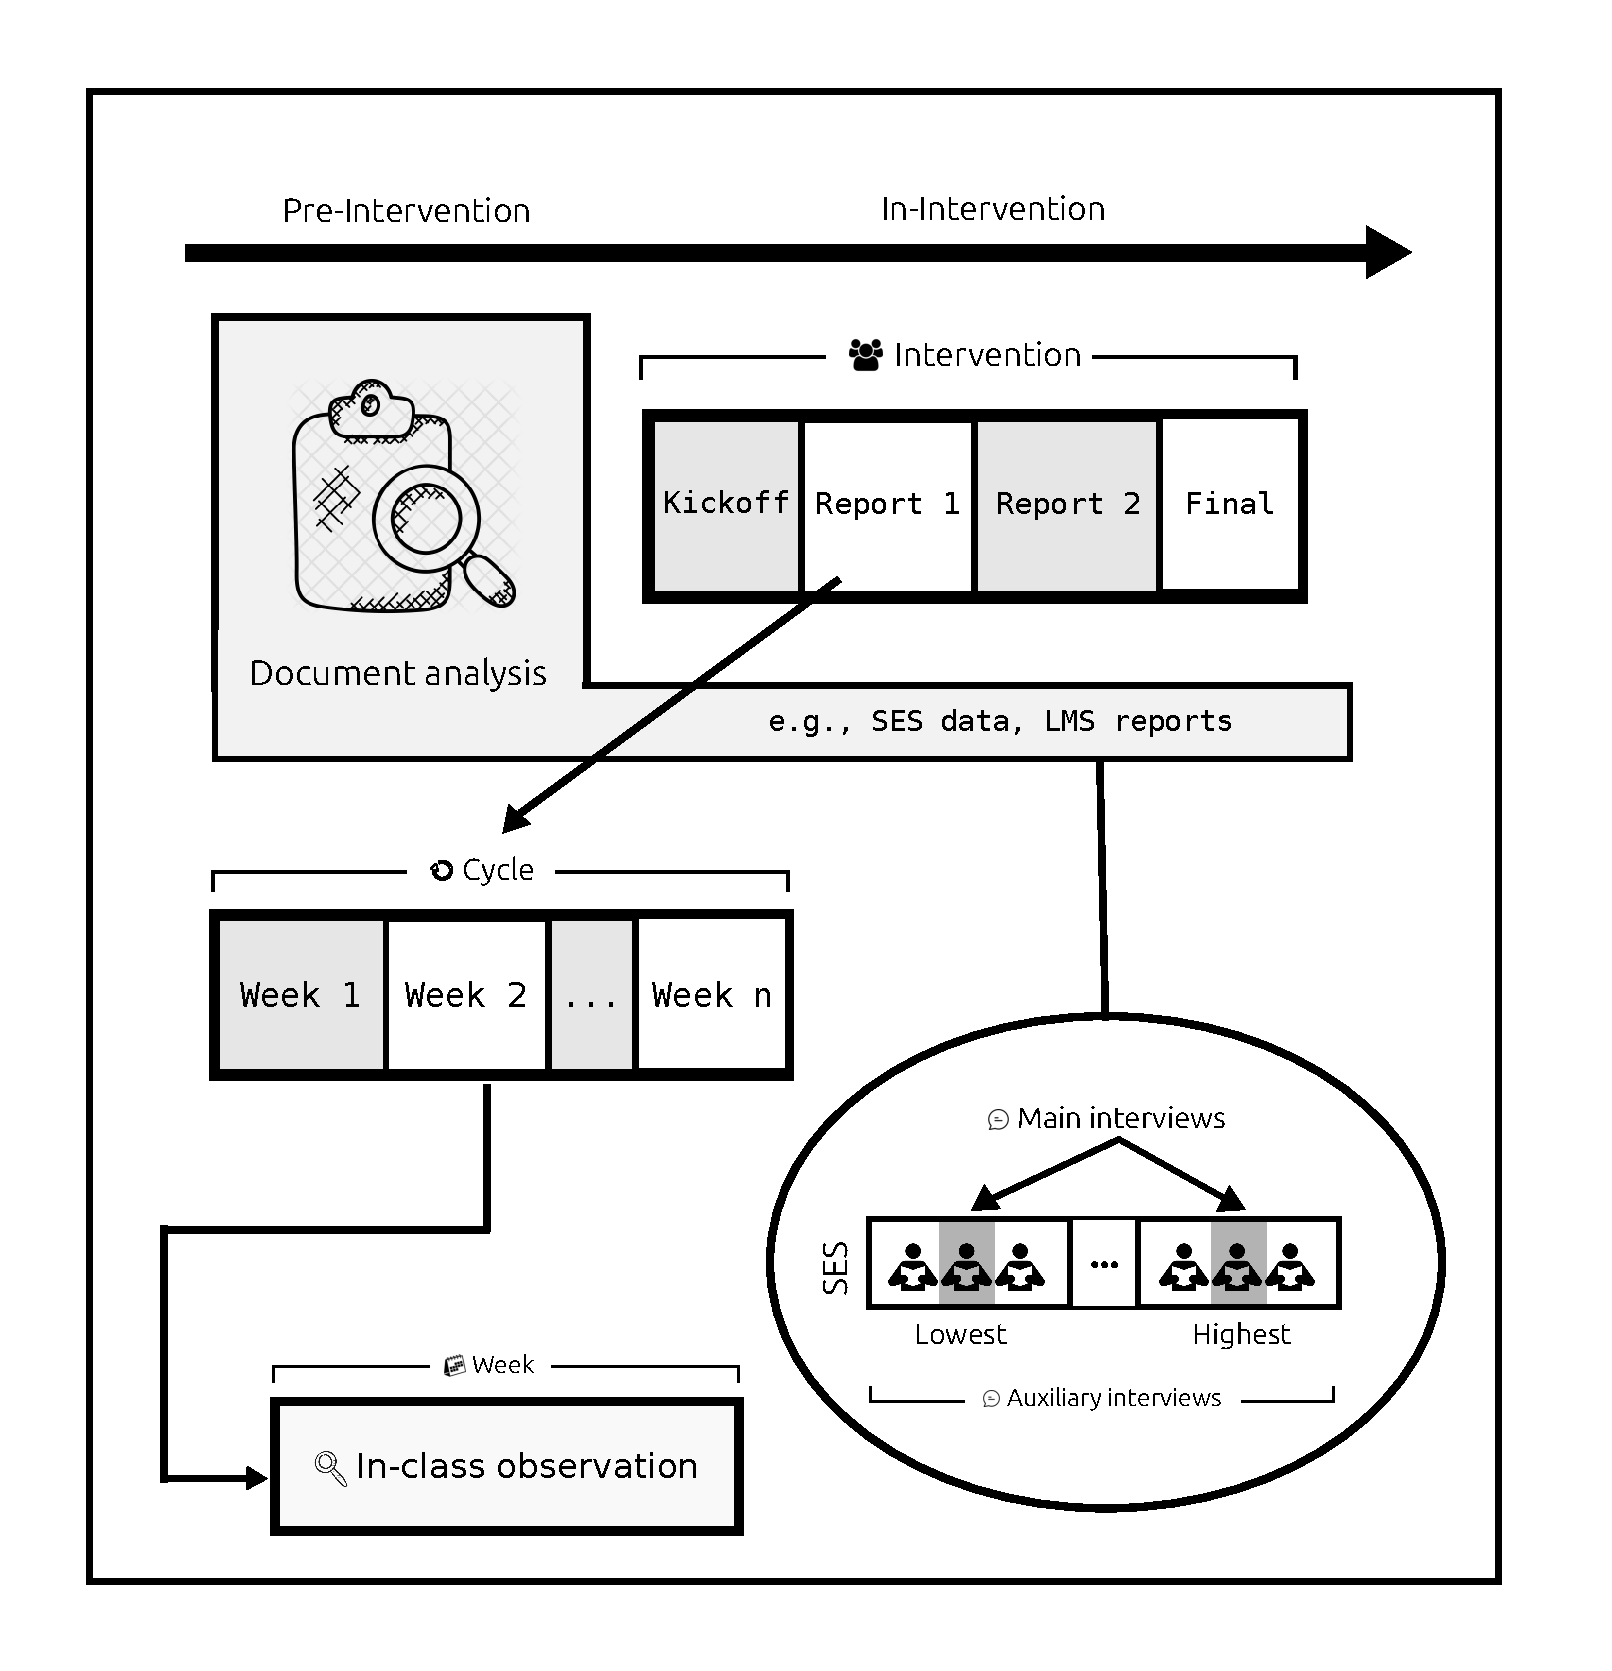
\includegraphics[width=0.9\textwidth]{images/chapter-07/new-methodology.pdf}}

\par\medskip\ABNTEXfontereduzida\selectfont\textbf{Source:} Created by the author (2024).
\end{figure}

As part of the consent and assent process, I presented my research project on May 30, 2023, during the first \gls{MIS} class. This presentation title was "Human Aspects in MIS"\footnote{Originally, "\textit{Aspectos Humanos em SGE}" in Brazilian Portuguese.}, lasting 40 minutes. The presentation comprised the following four topics: (i) introduction, (ii) notions on equity and ethics, (iii) research presentation, and (iv) consent for research\footnote{The presentation slides (in Brazilian Portuguese) are available on this \gls{Ph.D.} public repository: \url{https://github.com/bispojr/phd-info}.}. In the last topic, I avoided technical terms and concepts, focusing on showing the essence of research and all adopted care concerning research ethics involving humans, including current legal requirements \cite{bispojr:2021-wei}. I provided the informed consent form (and all ways to contact me during the research, in case of participation) for each student before this class (both on \gls{LMS} and repository). I kept the agreement of each student to participate in the research, counting on only those who answered me positively.

For students who voluntarily participated in the research (30 of 35 $\cong$ 85.71\% of \gls{MIS} class), I asked them to fill out a socioeconomic questionnaire (see Appendix \ref{chap:socio-quest}). This form allowed me to get socioeconomic information and plot the Lorenz curve from the average \acrfull{HPCI} data. This curve helped me to estimate the \gls{SES} of the class, stratifying them into four classes. Thus, all students belonged to a class alongside a continuum axis ranging between lower and higher \gls{SES} (see Section \ref{res-meth-ss:lorenz} and \ref{results-ss:classroom-data}). The idea was to pick two students and investigate these two ones during the term. I preferred to pick two students from the lowest and highest SES classes, respectively, aiming to understand if income disparity can be reflected in their capabilities. Another data source came from their classmates and other stakeholders, serving to triangulate and enrich the understanding of the research findings. Figure \ref{fig:participation-venn} presents in more detail the effective research participation of students in terms of \gls{ICF}, \gls{SQ}, and \gls{IP}.

\begin{figure}[ht!]
\centering

\caption{\textmd{Venn Diagram of the relations of three groups of students: those that (i) agreed with the \acrfull{ICF}, (ii) answered \acrfull{SQ}, and (iii) participated in interviews (\acrshort{IP}).}}
\label{fig:participation-venn}
\fcolorbox{gray}{white}{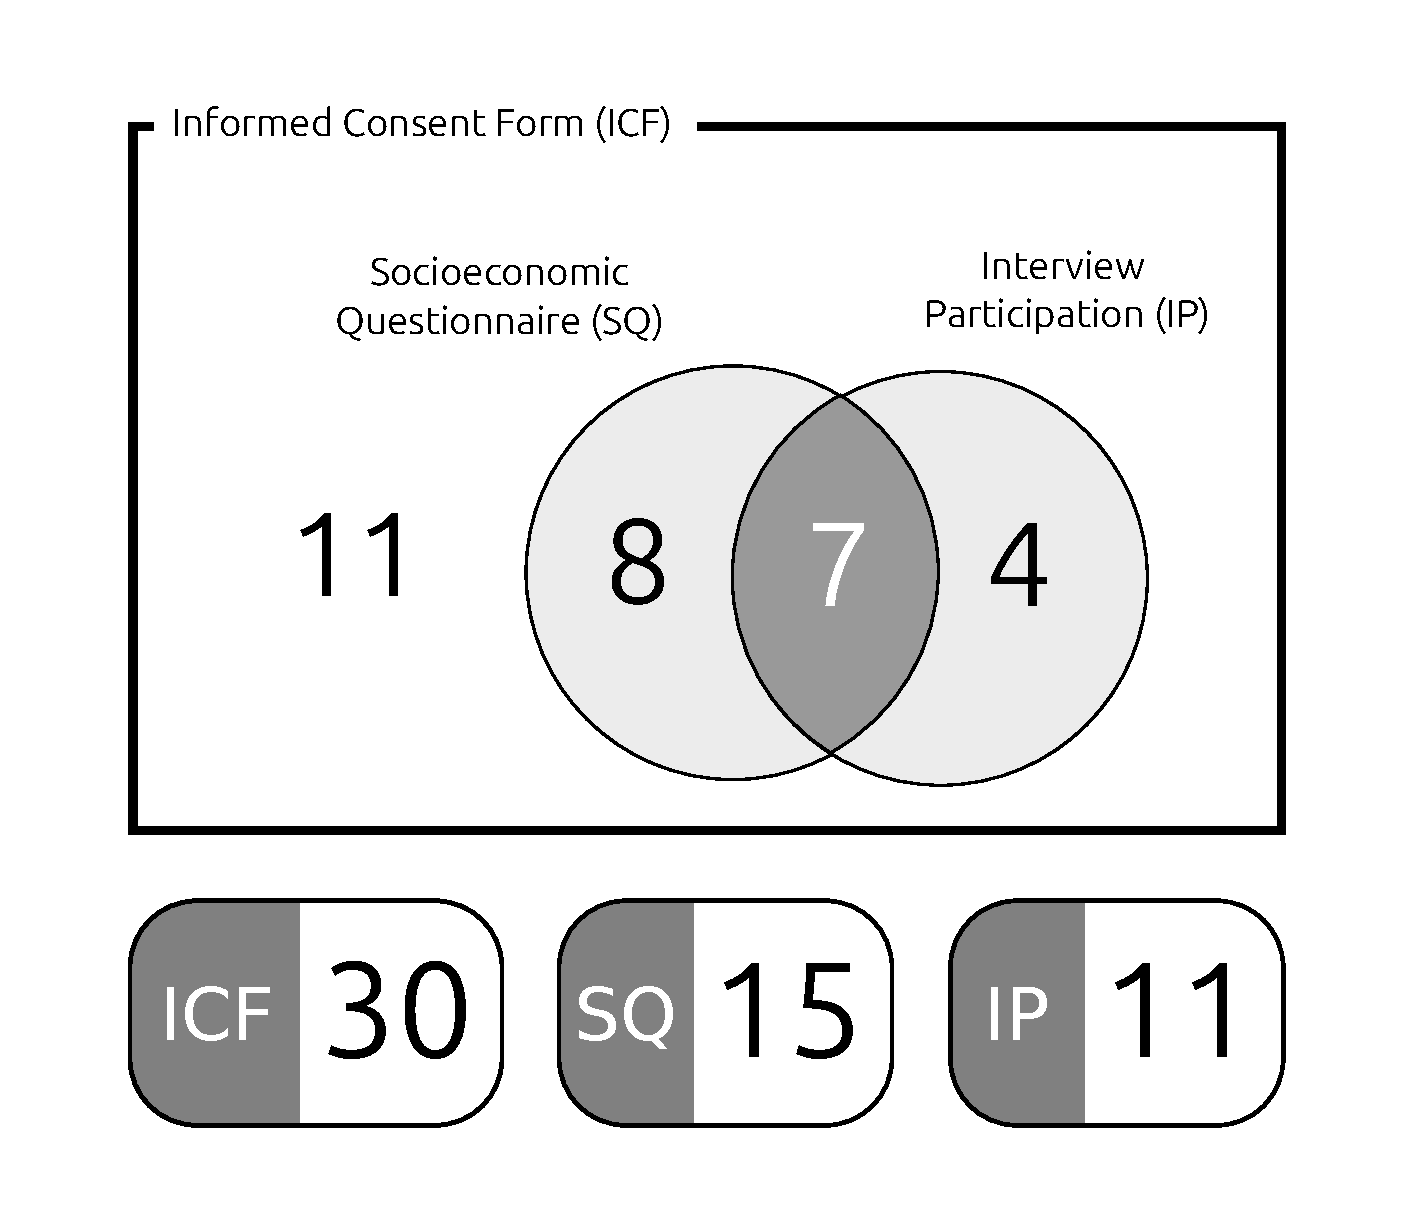
\includegraphics[width=0.9\textwidth]{images/chapter-07/participation.pdf}}

\par\medskip\ABNTEXfontereduzida\selectfont\textbf{Source:} Created by the author (2024).%\citeauthor{manualufpe2020} (\citeyear{manualufpe2020}) \par\medskip
\end{figure}

% \fbox{
%     \begin{minipage}[htb]{0.9\textwidth}
%         \vspace{0.3cm}
                
%         \colorbox{gray!30}{% create a colored box
%             \makebox[0.975\textwidth][l]{% center the text on the page
%                 \ \ \textbf{Further Writing}
%             }
%         }

%         \vspace{0.1cm}
        
%         \begin{itemize}
%             \item Describing first meeting (PBL planning).
%             \item Describing the research presentation (first day of class).
%             \item Describing the acceptance to participate in research, and interviews (included informed consent).
%             \item Creating a list of the date of interviews through a timeline term.
%         \end{itemize}

%         \vspace{0.25cm}
        
%     \end{minipage}
% }


\subsection{In-Intervention}
\label{phd-route-ss:in-int}

The second part of the second phase covers all effective activities to follow up the \gls{SDL} trajectories of \gls{CSE} students \textit{in situ} and remotely. This phase lasted five months, comprehending from the first (May 2023) to the last meeting with the integrated \gls{PBL} class (October 2023). I list the main activities that are: interviews, observation, and documental analysis. Figure \ref{fig:methodological-route} illustrates the whole intervention phase schematically. 

The interviews were the most important means of data collection. I conducted three blocks of interviews: the first one composed of three interviews (happening inside of Kickoff cycle), the second one composed of seven interviews (happening inside of Status Report 1 cycle), and the third one composed of a single interview (happening after the Final Report, see Table \ref{tbl:interview-dates}). The size of each block is different among themselves due to two reasons: (i) first, I conducted these interviews based on availability of each student (bearing in mind that this \gls{IS} program occurs at the night shift), and (ii) second, I opted to concentrate the most of interviews until the end of July 2023 because between August 2023 and January 2024 I was at Brunel University London in \gls{UK}, performing the Analysis \& Discussion phase also together to my co-advisor Prof. Marcus Vinicius De Matos (and I tried to offer the possibility for the interviewed could choose a in-person or remote format). Aiming to preserve the identity of each \gls{RP}, I use an alias like \gls{RP}4 to represent any research participant, and the aliases Chavo and Quico\footnote{Chavo and Quico are characters of Chespirito, a Mexican sitcom written by Roberto Bolaños. Chavo is the main character of Chespirito, a homeless person who sleeps inside a barrel. Quico is the son of Doña Florinda and a late naval captain. Chespirito presents him as a spoiled and overprotected 9-year-old-boy.} to represent the chosen participants from the lowest and highest \gls{SES} student groups (\gls{Q}1 and \gls{Q}4), respectively. I interviewed Chavo in the first block remotely, and Quico in the second block in-person. The semi-structured interview script is available in Appendix \ref{chap:appendix-scripts}.

\begin{table}[htb]
\caption{List of the three blocks of interviews indicating the period, \acrshort{PBL} cycle, and research participants.}
\label{tbl:interview-dates}
\centering
\rowcolors{1}{}{lightgray}
\begin{tabular}{
    m{3cm}|
    m{4cm}|
    m{4cm}|
    m{4cm}
}
    \hline
    \multicolumn{1}{c|}{
        \textbf{Block} 
    } &
    \multicolumn{1}{c|}{
    \textbf{Participants}
    } &
    \multicolumn{1}{c|}{
    \textbf{Period}
    } &
    \multicolumn{1}{c}{
    \textbf{Cycle}
    } \\
    
    \hline
    \multicolumn{1}{c|}{
        1
    } &
    \multicolumn{1}{c|}{
        RP1-2, Chavo
    } &
    \multicolumn{1}{c|}{
        May 30 to Jun 22
    } &
    \multicolumn{1}{c}{
        Kickoff
    } \\

    \multicolumn{1}{c|}{
        2
    } &
    \multicolumn{1}{c|}{
        RP3-8, Quico
    } &
    \multicolumn{1}{c|}{
        Jun 23 to Jul 25
    } &
    \multicolumn{1}{c}{
        Status Report 1
    } \\

    \multicolumn{1}{c|}{
        3
    } &
    \multicolumn{1}{c|}{
        RP9
    } &
    \multicolumn{1}{c|}{
        After Sep 21
    } &
    \multicolumn{1}{c}{
        After Final Report
    } \\
    \hline
    % \hline
    % \multicolumn{2}{c}{Item of Information} &
    % Related \gls{DSRQ}\\
    % \hline
    % Research &
    % Type & \gls{DSRQ}.1 \\
    % & Kind & \gls{DSRQ}.1 \\
    % & Methodology & \gls{DSRQ}.1 \\
    % \hline
    % Context &
    % Educational Level & \gls{DSRQ}.2 \\
    % & Country / Region & \gls{DSRQ}.2 \\
    % \hline
    % Equity & 
    % Equity Issue & \gls{DSRQ}.3 \\
    % & General Equity Theory / Framework & \gls{DSRQ}.3 \\
    % \hline
    % - &
    % Active Learning Approach & \gls{DSRQ}.4\\
    % \hline
    
\end{tabular}

\par\medskip\ABNTEXfontereduzida\selectfont\textbf{Source:} Created by the author (2024). \par\medskip

\end{table}

The observation was conducted during some collective activities in the class. In summary, these activities encompassed all classes of three courses and all integrated presentations in the final of each cycle (Kickoff, Status Reports 1 and 2, and Final Report), focusing my attention on \gls{MIS} course. I obtained access to all forums, both those with only student access and those with professors and tutors (who talked among them privately). I also took reflexivity notes continuously. This observation data guided me in choosing what student in each group I should prioritize to interview, for instance. Other different data sources could contribute to reinforcing the confluence of a finding or even significantly contrasting it, leading me to pay attention to certain aspects that previously were unconsidered. 

The documental analysis also was important over the intervention phase. During the integrated \gls{PBL} course, students made several documents in groups or individually. Some of these were deliverable artifacts required to be submitted in \gls{LMS} (or done in-person) at each cycle ending (e.g., \gls{UML} diagrams, slides, reports, exams). Other part consisted of form responses that each student helped the professors and tutors informing about the quality of the \gls{PBL} approach (e.g., \gls{PBL} tests, group and concept feedback). The data available from the open educational repositories and institutional databases were useful to situate the observed and reported conditions into a broader scenario both in \gls{UFPE} and in \gls{IS} class.%the institution and even the country.

%{\color{red} Lastly, I can trigger the focus group on specific occasions. In the cycle endings, a focus group can reveal key information about the capabilities that arise more naturally in a group setting instead of an individual one. Thus, the idea is to investigate capability aspects that emerge in a collective context. Furthermore, eventual mismatches can be identified between the individual and group perceptions. The semi-structured script of the focus group is available in  Appendix A3 (Table A3.2)}.


\subsection{Analysis \& Discussion}
\label{phd-route-ss:ana-dis}

The third (and last) phase covers all activities and decisions responsible for analyzing and discussing the research results. This phase lasted nearly 12 months, comprehending from the last meeting with the integrated \gls{PBL} class (October 2023) to the submission of this \gls{Ph.D.} thesis for examining committee appreciation (October 2024). I list the main activities: guidelines structuring, interview coding, document organization, data aggregation, and thesis writing completion.

After the qualifying project presentation, I received a precious feedback in a question format: "What would it be the research relevance to \gls{CEd} practitioners?"\footnote{I presented the research relevance to \gls{CEd} practitioners in Section \ref{intro-sec:rel-computing}.}. This feedback led me to include \gls{RG}3 seeking recommending guidelines to (\gls{CSE}) educational stakeholders concerning how to consider effectively equity issues and active learning from the \acrfull{CA} lens. To be honest, a seed of these guidelines had been discussed for us previously (before the qualifying project presentation) problematizing the \gls{CEd} neutrality presupposition \cite{bispojr:2022-educomp}. When I realized that this essay was the first document of guidelines, thus the next steps were to structure how to discuss equity effectively in \gls{CEd} decision-making collective of teachers (including \gls{CSE} perspective too).

Before the opportunity to submit a Springer chapter proposal for a book of \gls{OLEE}, my advisors and I decided to expand the scope of these guidelines to Engineering Education, providing a set of guiding questions to orientate an initial equity analysis for an Engineering decision-making collective of professors \cite{bispojr:2024-online-lab}. Bearing in mind that \glspl{LLM} started to be included as a new challenge in several educational contexts, I participated in the \gls{NMP} Conference talking about \gls{CEd}, equity, and \glspl{LLM}. In a second moment, my advisors and I extended this presentation ideas providing constructs to analyze equity in a computing class from our new concept of \gls{LLM} divide using \gls{CA} lens \cite{bispojr:2024-nmp}. These two contributions were written during my academic visit to Brunel University London.

After choosing the participants Chavo and Quico, I performed their interview coding. I used the Notion platform\footnote{See in \url{http://www.notion.so}.} to manage the codes, putting the little blocks of transcript interviews in a table column and the codes in another one. I conducted three big coding rounds, having several iterations into each round: (i) first round to code the main \gls{SDL} constructs (Section \ref{res-sec:interviews}), (ii) second round to code from \gls{SDL} goals and \gls{SSDL} perspective (\gls{RG}1, see Section \ref{disc-sec:sdl-trajectories}), and (iii) third round to code from \gls{SDL} capabilities\footnote{\gls{SDL} capabilities is a new concept that I created to establish the meeting between \gls{SDL} and \gls{CA} constructs. See more in Section \ref{disc-sec:sdl-capabilities}.} (\gls{RG}2, see Section \ref{disc-sec:sdl-capabilities}). It is important to note that I had the opportunity to join as a member of \gls{HDCA}\footnote{See \gls{HDCA} website: \url{https://hd-ca.org/}.}, participating more specifically in \gls{HDCA} Education Thematic Group. I was mentored by Prof. Monica Kuwahara from \gls{UFABC} since March 2024 in \gls{HDCA} Early Career Researchers and Practitioners Network Mentorship Program 2023-24\footnote{See more detail in \url{https://hd-ca.org/thematic_group/early-career-researchers-practitioners-network}.}. She is also one of the \gls{HDCA}'s coordinators for the Regional Network of Latin America, helping me to understand better about the application of \gls{CA} constructs.

The document organization was an activity to collect and arrange all related documents that were relevant to enlighten the interview findings. I divided into three document groups: curricula, \gls{UFPE} open data, and \gls{IS} class records. I detail each one in Section \ref{res-sec:context-overview}.

The data aggregation occurred in a posterior moment in relation to the document organization aiming to create charts to visualize the overall picture from each level of analysis (e.g., \gls{PBL} team, class, program, university). For instance, I put in Appendix \ref{chap:pbl-see-charts} all charts extracted from five elements of \gls{PBL-SEE}, locating Chavo and Quico in their respective \gls{PBL} team or even in their whole \gls{IS} class. The underlying idea is to realize the overall context for both participants, trying to capture some collective determinants for each one of them.

Lastly, in this phase, I finished the thesis writing. To be sure, the thesis writing was a continuous activity that started from the early phases of my \gls{Ph.D.} route. A significant part of my thesis came from the qualifying project, introducing new theoretical insights, adjusting the methodological design, and, mainly, presenting (Chapter \ref{chap:results}) and discussing (Chapter \ref{chap:discussion}) the results.

Frame \ref{frame:research-design} summarizes some research design choices in this chapter.

%a diferença do quadro pra tabela é que o quadro tem linhas verticais
\begin{quadro}
\caption{Main research design choices.}
\label{frame:research-design}
\centering
\begin{tabular}{|l|l|}
\cline{1-2}

\textbf{Research Context} & 
Information System 2023.1, \gls{MIS} Course \\
\hline

\multirow{2}{*}{\textbf{Number of Interviews}} &
 Main Interviews (2)\\
 & Auxiliary Interviews (9)\\
 \hline
 \textbf{Active Learning Approach} &
 PBL By-Cycles Framework \cite{alexandre:2018}\\
 \hline
 \textbf{Active Learning Construct} &
 Self-Directed Learning \cite{knowles:1975,grow:1991}\\
 \hline
 \textbf{Equity Theory} &
 Capability Approach \cite{sen:1992}\\
\hline

%A& B &  C& D &E  \\ \cline{1-5}
%\multirow{3}{*}{1}  & 2 &  3& 4& 5 \\
% &  2 &  3& 4& 5  \\
% &  2 &  3& 4& 5 \\
% \cline{1-5}
\end{tabular}
  \par\medskip\ABNTEXfontereduzida\selectfont\textbf{Source:} Created by the author (2024). \par\medskip
\end{quadro}

% \fbox{
%     \begin{minipage}[htb]{0.9\textwidth}
%         \vspace{0.3cm}
                
%         \colorbox{gray!30}{% create a colored box
%             \makebox[0.975\textwidth][l]{% center the text on the page
%                 \ \ \textbf{Further Writing}
%             }
%         }

%         \vspace{0.1cm}
        
%         \begin{itemize}
%             \item Remember to put the guidelines here.
%             \item Presenting better this phase:
%             \begin{itemize}
%                 \item Codifying all the transcripts of interviews.
%                 \item Triangulating the data against other sources of data (e.g., document, observational data, in-between interviews).
%                 \item Conducting thematic analysis.
%                 \item Specifying how to get the capabilities cartography.
%                 \item Writing the final report.
%             \end{itemize}

%         \end{itemize}

%         \vspace{0.25cm}
        
%     \end{minipage}
% }